\section{Numerical experiments}
\label{ch:num}
We present numerical examples\footnote{All test cases are publicly available from the author's \href{https://github.com/ManuelMBaumann/elastic_benchmarks}{github} repository \cite{Bgithub}.} for the two-dimensional, elastic \marmousi model \cite{marm2} as well as for a three-di\-men\-sional elastic \texttt{wedge} problem which has been inspired by the well-known acoustic test case introduced in \cite{Knibbe2016,PM04} for 2D and 3D, respectively. In the examples, we restrict ourselves to Cartesian grids with fixed discretization size \mbox{$h \equiv h_x = h_y = h_z$}. Depending on the specific problem parameters, the maximum frequency we allow is restricted by,
\begin{align*}
f_\text{max} < \frac{\text{min}_{\mathbf{x} \in \Omega}\{c_p,c_s\}}{ppw \cdot h}, \quad ppw = 20,
%  ppw = \frac{\lambda_{\text{min}}}{h}, \quad \text{with } \lambda_{\text{min}} = \frac{\text{min}\{c_{p,s}(\mathbf{x})\}}{f_\text{max}}
\end{align*}
where in the following experiments a minimum of $20$ points per wavelength ($ppw$) is guaranteed, and $\omega_k = 2 \pi f_k$.

All numerical examples presented in this section have been implemented in FORTRAN 90
using the GNU/gfortran compiler running over GNU/Debian Linux, and executed on a computer with 
4 CPUs Intel I5 with 32 GB of RAM.
\subsection{Parameter studies}
 We begin our numerical tests with a sequence of experiments performed on an \textit{academic} two-dimensional \texttt{wedge} problem described in Figure \ref{fig:wedge2d}. The aim of these first experiments is to prove the following concepts for the 2D algorithm introduced in Section \ref{ch:msss_lu}:
 \begin{itemize}
  \item Demonstrate the dependency of the iterative solution meth\-od on the maximum off-di\-ag\-o\-nal rank, $r^\ast = \max \{ r^l, r^u\}$. In Experiment \ref{exp:off_rank} we show that a small value of $r^\ast$ leads to a very good preconditioner in terms of number of Krylov iterations.
  \item Show that the 2D algorithm yields linear computational complexity when all problem parameters are unchanged and the grid size doubles (Experiment \ref{exp:lin_compl}).
  \item In Experiments \ref{exp:freq1} and \ref{exp:freq2}, we evaluate the frequency dependency of the MSSS-preconditioner \eqref{eq:precon} when $\tau \neq \omega$. This is in particular important when multiple frequencies in a matrix equation framework are considered in Section \ref{ch:best_tau}.
 \end{itemize}
 
\begin{figure}[H]
  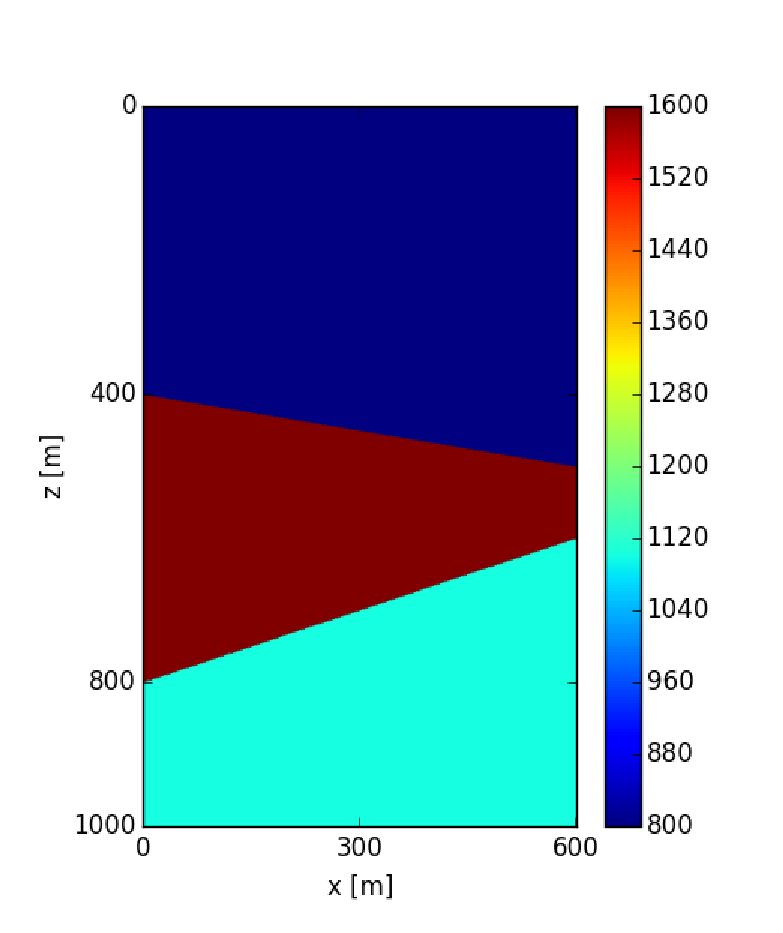
\includegraphics[width=0.49\columnwidth]{wedge2d_cs} \hfill
  \includegraphics[width=0.49\columnwidth]{wedge2d_uz}
\caption{2D elastic \texttt{wedge} problem used for parameter study: Speed of S-waves in $m/s$ (left) and real part of $z$-component of displacement vector at $f = 16$ Hz (right).}
\label{fig:wedge2d}
\end{figure}

We perform parameter studies on a two-dimensional slice ($xz$-plane) of the \texttt{wedge} problem described in Figure \ref{fig:wedge3d_par}. The values of $\rho, c_p$ and $c_s$ in the respective layers are given in Table \ref{tab_params}, and the considered computational domain $\Omega = [0,600] \times [0,1000]$ meters is shown in Figure \ref{fig:wedge2d}.

\begin{table}[ht]
\centering
 \caption{Parameter configuration of the elastic \texttt{wedge} problem. The Lam\'e parameters can be computed via \eqref{eq:lame}.} \label{tab_params} 
 \begin{tabular}{|l|c|c|c|}
 \hline
  Parameter & Layer \#1 & Layer \#2 & Layer \#3 \\
  \hline
  $\rho [kg/m^3]$ & 1800& 2100&1950 \\
  $c_p [m/s]$ & 2000&3000 & 2300\\
  $c_s [m/s]$ & \phantom{0}800&1600&1100 \\
  \hline
 \end{tabular}
\end{table}

% \subsubsection{Single-frequency case}
In the first set of experiments, we restrict ourselves to the single-frequency case, $\Nom = 1$. The discrete problem is, thus, given by,
\begin{align*}
 (K + i \omega C - \omega^2 M) \x = \rhs,
\end{align*}
with a preconditioner that approximates the original operator, $\mathcal{P}(\tau) \approx (K + i \tau C - \tau^2M),  \tau = \omega$, by taking low-rank approximations in the block-LU factorization.  

\begin{exper}[Off-diagonal rank] \label{exp:off_rank}
This experiment evaluates the performance of the MSSS-preconditioner \eqref{eq:perm_precon} for 2D problems when the maximal off-diagonal rank $r^\ast$ is in\-creased. 
\end{exper}
In Experiment \ref{exp:off_rank}, we apply the approximate block-LU decomposition \eqref{eq:full_Schur}-\eqref{eqn_schur} as described in Section \ref{ch:msss_lu} to the 2D \texttt{wedge} problem at frequencies $f=8$ Hz and $f=16$ Hz. The maximum off-diagonal rank $r^\ast = \max \{ r^l, r^u\}$ of the Schur complements \eqref{eqn_schur} is restricted using model order reduction techniques, cf. \cite{QG15}. The dimension of the diagonal constructors has been chosen to be $m_i = 40$, cf. Table \ref{tab_sss_size}. Figure~\ref{fig:exp1} shows the convergence behavior of preconditioned  IDR($4$) (Algorithm \ref{bio_idr} with $\Nom =1$) and preconditioned BiCGStab \cite{v92}. We note that even in the high-frequency case, an off-di\-ag\-o\-nal rank of $r^\ast = 10$ leads to a very efficient preconditioner, and an (outer) Krylov method that converges within at most $40$ iterations to a residual tolerance \texttt{tol=10e-8}. Moreover, we observe that IDR($s$) outperforms BiCGStab in the considered example when the same preconditioner is applied. For a rank $r^\ast > 15$, we observe convergence within very few iterations.
\begin{figure}[H]
  \includegraphics[width=\columnwidth]{order_2d_new.pdf}  
\caption{Number of Krylov iterations when the maximum off-diagonal rank of the inverse Schur complements is restricted to $r^\ast$.}
\label{fig:exp1}
\end{figure}

\begin{exper}[Computational complexity in 2D] \label{exp:lin_compl}
The inexact block-LU factorization yields linear computational complexity when applied as a preconditioner within MSSS-pre\-conditioned IDR($s$), demonstrated for the 2D wedge problem.
\end{exper}
In our second numerical experiment, the maximum off-di\-ag\-o\-nal rank is fixed to $r^\ast =15$ such that very few IDR iterations are required, and the computational costs in Figure \ref{fig:exp:linCompl} are dominated by the MSSS preconditioner. We solve the 2D \texttt{wedge} problem at frequency $8$ Hz for different mesh sizes and a finite element discretization with B-splines of degree $p = \{1,2\}$. In Figure \ref{fig:exp:linCompl}, the CPU time is recorded for different problem sizes: The mesh size $h$ is doubled in both spatial directions such that the number of unknowns quadruples according to \eqref{eq:unknows}. From our numerical experiments we see that the CPU time increases by a factor of $\sim 4$ for both, linear and quadratic, splines. This gives strong numerical evidence that the 2D MSSS computations are performed in linear computational complexity.

\begin{figure}[ht]
  \includegraphics[width=\columnwidth]{draw_fig_new2.pdf}
\caption{Linear computational complexity of preconditioned IDR($4$) for the 2D \texttt{wedge} problem at $f=8$ Hz.}
\label{fig:exp:linCompl}
\end{figure}

\begin{exper}[Constant points per wavelength] \label{exp:freq1}
Conver- gence behavior of MSSS-preconditioned IRD($s$) when the problem size and wave frequency are increased simultaneously.
\end{exper}
In the previous example, the wave frequency is kept constant while the problem size is increased which is of little practical use due to oversampling. We next increase the wave frequency \textit{and} the mesh size simultaneously such that a constant number of points per wavelength, $ppw=20$, is guaranteed.
\begin{table}[ht]
\centering
 \caption{Performance of the MSSS preconditioner when problem size and frequency are increased simultaneously such that $ppw = 20$ and \texttt{tol=10e-8}: $\mathcal{O}(n^3)$ complexity.} \label{tab_freq_indep} 
 \begin{tabular}{|c|c|c|c|c|c|}
 \hline
  $f$ & $h [m]$ & $r^\ast$ & MSSS & IDR($4$) & total CPU time\\
  \hline
  $\phantom{0}4$ Hz & $10.0$& \phantom{0}5& 0.55 sec& \phantom{0}16 iter.& \phantom{0}0.71 sec\\
  $\phantom{0}8$ Hz & $\phantom{0}5.0$& \phantom{0}7 & 2.91 sec& \phantom{0}33 iter.& \phantom{00}4.2 sec \\
  $16$ Hz & $\phantom{0}2.5$& 10 &  15.3 sec& \phantom{0}62 iter.& \phantom{0}31.8 sec\\
  $32$ Hz & $1.25$& 16& 95.4 sec&101 iter. & 242.5 sec\\
  \hline
 \end{tabular}
\end{table}
In Table \ref{tab_freq_indep}, we use the freedom in choosing the maximum off-diagonal rank parameter $r^\ast$ such that the overall preconditioned IDR($s$) algorithm converges within a total number of iterations that grows linearly with the frequency.  This particular choice of $r^\ast$ shows that the MSSS preconditioner has comparable performance to the multi-grid approaches in \cite{Plessix2007,Rizzuti2016} where the authors numerically prove $\mathcal{O}(n^3)$ complexity for 2D problems of size $n_x = n_y \equiv n$.

The off-diagonal rank parameter $r^\ast$ can on the other hand be used to tune the preconditioner in such a way that the number of IDR iterations is kept constant for various problem sizes. In Table \ref{tab_freq_indep2}, we show that a constant number of $\sim 30$ IDR iterations can be achieved by a moderate increase of $r^\ast$ which yields an algorithm that is nearly linear.
\begin{table}[ht]
\centering
 \caption{Performance of the MSSS preconditioner when problem size and frequency are increased simultaneously such that $ppw = 20$ and \texttt{tol=10e-8}: Constant number of iterations.} \label{tab_freq_indep2}
 \begin{tabular}{|c|c|c|c|c|c|}
 \hline
  $f$ & $h [m]$ & $r^\ast$ & MSSS & IDR($4$) & total CPU time\\
  \hline
  $\phantom{0}4$ Hz & $10.0$& \phantom{0}3 & \phantom{0}0.50 sec & 29 iter.& \phantom{0}0.83 sec\\
  $\phantom{0}8$ Hz & $\phantom{0}5.0$& \phantom{0}7 &  \phantom{0}2.91 sec & 33 iter.& \phantom{00}4.2 sec \\
  $16$ Hz & $\phantom{0}2.5$& 11 & \phantom{0}16.9 sec& 27 iter.& \phantom{0}24.5 sec\\
  $32$ Hz & $1.25$& 18& 107.1 sec & 33 iter. & 163.2 sec\\
  \hline
 \end{tabular}
\end{table}

\begin{exper}[Quality of $\mathcal{P}_{2D}(\tau)$ when $\tau \neq \omega$] \label{exp:freq2}
Single-fre- quency experiments when seed frequency differs from the original problem. 
\end{exper}

\begin{figure}[H]
  \includegraphics[width=\columnwidth]{iter_vs_tau_new.pdf}  
\caption{Number of iterations of preconditioned IDR($s$) when $\tau \neq \omega$ in \eqref{eq:perm_precon}. We perform the experiment for different frequencies, and keep a constant grid size $h=5m$ and residual tolerance \texttt{tol = 10e-8}.}
\label{fig:iter_vs_tau}
\end{figure}

This experiments bridges to the multi-frequency case. We consider single-frequency problems at $f \in \{2,3,4,5\}$~Hz, and vary the parameter $\tau$ of the preconditioner \eqref{eq:perm_precon}. The off-diagonal rank $r^\ast$ is chosen sufficiently large such that fast convergence is obtained when $\tau = \omega$. From Figure \ref{fig:iter_vs_tau} we conclude that the quality of the preconditioner heavily relies on the seed frequency, and a fast convergence of preconditioned IDR($4$) is only guaranteed when $\tau$ is close to the original frequency.

% \subsubsection{Multi-frequency case}
\subsection{The elastic \marmousi model}
\label{ch:best_tau} 
We now consider the case when $\Nom > 1$, and the matrix equation,
\begin{align}
\label{eq:me2}
K \X + i C \X \Sigma - M \X \Sigma^2 = \blkrhs, \quad \X \in \mathbb{C}^{\n \times \Nom},
\end{align}
is solved. Note that this way we can incorporate multiple wave frequencies in the diagonal matrix $\Sigma = \text{diag}(\omega_1,...,\omega_\Nom)$, and different source terms lead to a block right-hand side of the form $\blkrhs = [\rhs_1,...,\rhs_\Nom]$. When multiple frequencies are present, the choice of seed frequency $\tau$ is crucial as we demonstrate for the \marmousi problem in Experiment~\ref{multifreq}.
% \subsection{The elastic \marmousi model}
We solve the matrix equation \eqref{eq:me2} arising from the realistic \marmousi problem \cite{marm2}. We consider a subset of the computational domain, $\Omega = [0,4000] \times [0,1850] m$, as suggested in \cite{Rizzuti2016}, cf. Figure \ref{fig:marm}.

\begin{exper}[\marmousi at multiple right-hand sides]\label{multiRHS}
Per\-for\-mance of the MSSS-preconditioned IDR(s) method for the two-dimensional \marmousi problem when multiple source locations are present.
\end{exper}
We consider the \marmousi problem depicted in Figure~\ref{fig:marm} at $h=5$m and frequency $f=2$ Hz. We present the performance of MSSS-preconditioned IDR($4$) for $\Nom$ e\-qually-spaced source locations (right-hand sides) in Table \ref{tab_mar2}. The CPU time required for the preconditioner as well as the iteration count is constant when $\Nom > 1$ because we consider a single frequency. The overall wall clock time, however, scales better than $\Nom$ due to the efficient implementation of block matrix-vector products in the IDR algorithm. The experiment for $\Nom=20$ shows that there is an optimal number of right-hand sides for a single-core algorithm.

 \begin{table}[H]
 \caption{Numerical experiments for the \marmousi problem at $f=2$ Hz using a maximum off-diagonal rank of $r^\ast=15$.} \label{tab_mar2}
  \centering
  \begin{tabular}{|c|c|c|}
  \hline
   \# RHSs & MSSS fact. [sec] & IDR(4) [sec]\\
   \hline
   1 & 60.2 & \phantom{0}8.18  (8 iter.) \\
   5 & 60.2 & \phantom{0}25.0 (8 iter.) \\
   10 & 60.1  &\phantom{0}43.5 (8 iter.)\\
   20 & 60.3 &  108.3 (8 iter.) \\
   \hline
  \end{tabular}
 \end{table}

\begin{figure}[H]
  \includegraphics[width=0.98\columnwidth]{cs-crop.eps}\\
  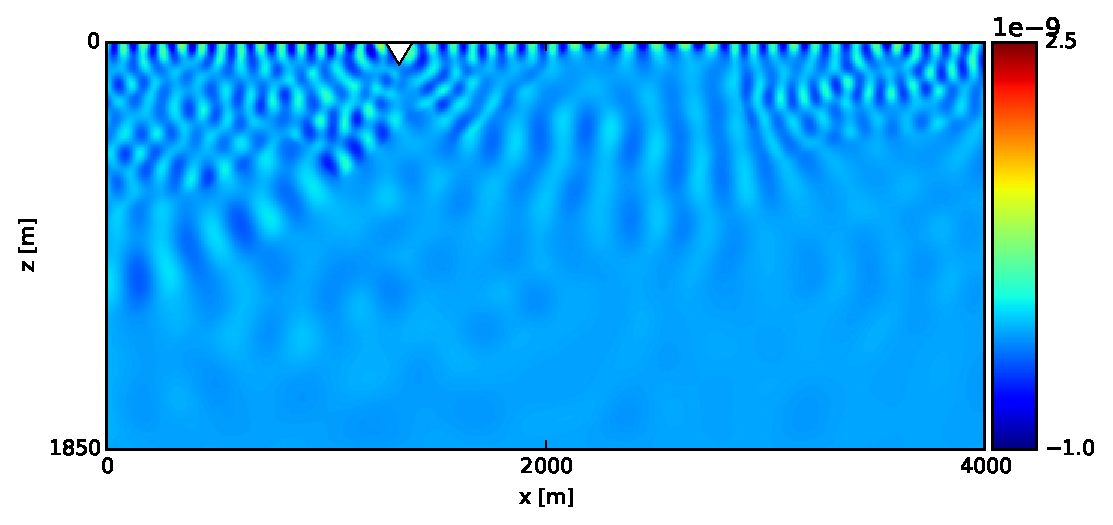
\includegraphics[width=0.98\columnwidth]{disp_z10_f4-crop.eps}\\
  \includegraphics[width=0.98\columnwidth]{disp_z10_f6-crop.eps}

\caption{Speed of S-waves in $m/s$ (top), and real part of the $z$-component of the displacement vector in frequency-domain at $f=4$ Hz (middle) and $f=6$ Hz (bottom) for the \marmousi model, cf. \cite{marm2} for a complete parameter set. The source location is indicated by the symbol '$\triangledown$'.}
\label{fig:marm}
\end{figure}

\begin{exper}[\marmousi at multiple frequencies]\label{multifreq}
Per\-for\-mance of MSSS-preconditioned IDR(s) for the two-di\-men\-sional \marmousi problem at multiple frequencies.
\end{exper}

 \begin{figure}[H]
 \centering
  \includegraphics[width=0.6\columnwidth]{ms_time.pdf}
%   \includegraphics[width=0.6\columnwidth]{ms_rot_new.pdf}
  \caption{Total CPU times of MSSS-IDR($4$) for $\Nom > 1$ frequencies equally-spaced within a fixed range. Additional scaling (dashed lines) following \cite{BvG17} improves convergence, and allows for larger frequency ranges.}\label{fig:multiF}
 \end{figure}
 In Experiment \ref{multifreq}, we consider a single source term located at $(L_x/2,0)^\mathsf{T}$ and $\Nom$ frequencies equally-spaced in the intervals $f_k \in [2.4,2.8]$ Hz and $f_k \in [2.0,4.0]$ Hz. The seed frequency is chosen at $\tau = (1-0.5i)\omega_{max}$ for which we recorded optimal convergence behavior. When the number of frequencies is increased, we observe an improved performance compared to an extrapolation of the $\Nom=2$ case. We also observed that the size of interval in which the different frequencies range is crucial for the convergence behavior. In~\cite{BvG17}, we describe how the convergence of global \mbox{GMRES \cite{JMS99}} can be improved by scaling the $k$-th column of the block unknown $\mathbf{X}$ by $e^{-i\varphi_k}$. Spectral anlysis shows that the angles $\varphi_k$ can be chosen such that the spectrum of the preconditioned operator is rotated and convergence is improved, cf. \cite{BvG17}.  In the present case of global IDR($s$) (Algorithm \ref{bio_idr}) combined with an inexact MSSS preconditioner \eqref{eq:perm_precon} we record a reduction to $60\%$ of the CPU time when spectral rotation is applied to the $\Nom=10$ case, cf. Figure~\ref{fig:multiF}.
\subsection{A three-dimensional elastic \texttt{wedge} problem}
\label{ch:wedge3d}
The \texttt{wedge} problem with parameters presented in Table \ref{tab_params} is extended to a third spatial dimension, resulting in $\Omega = [0,600] \times [0,600] \times[0,1000] \subset \mathbb{R}^3$.
\begin{figure}[ht]
  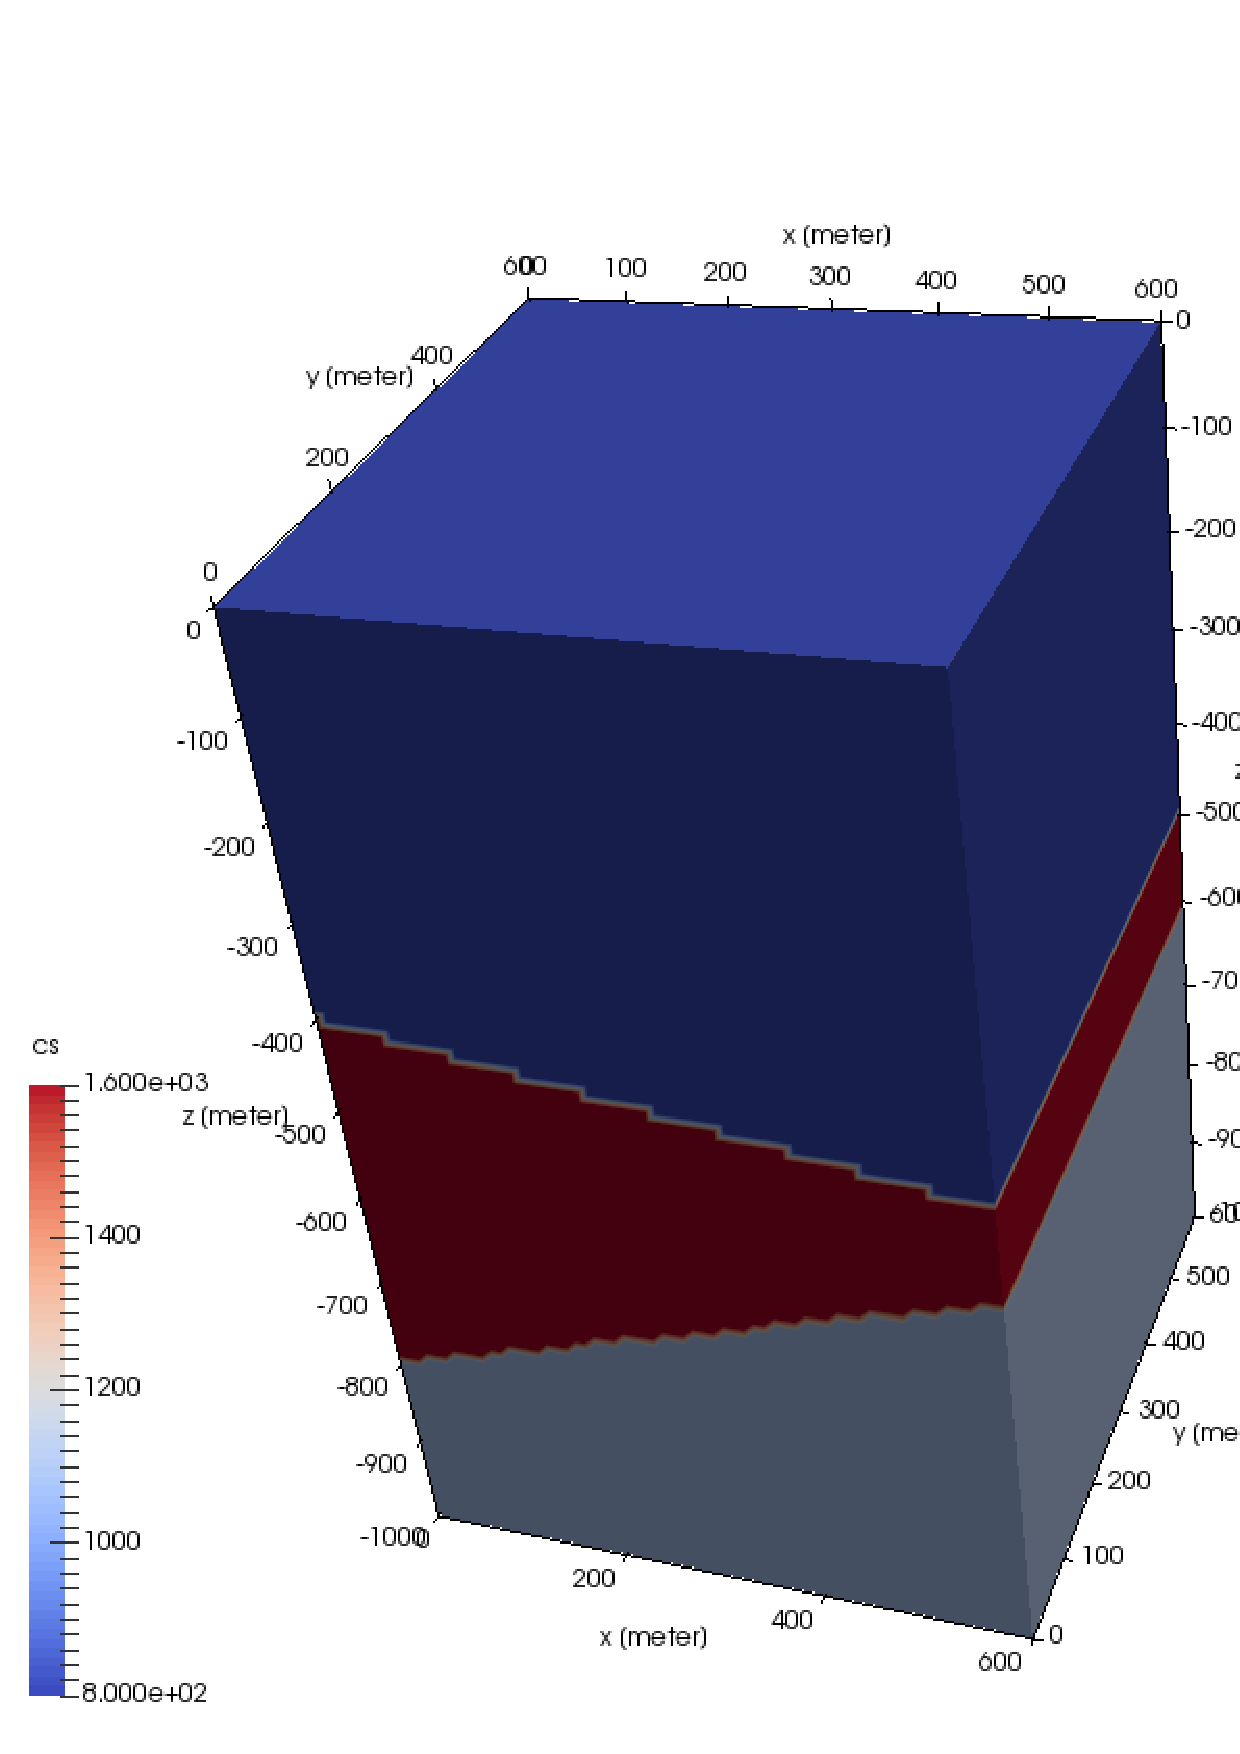
\includegraphics[width=0.49\columnwidth]{wedge3d_cs.png} \hfill
  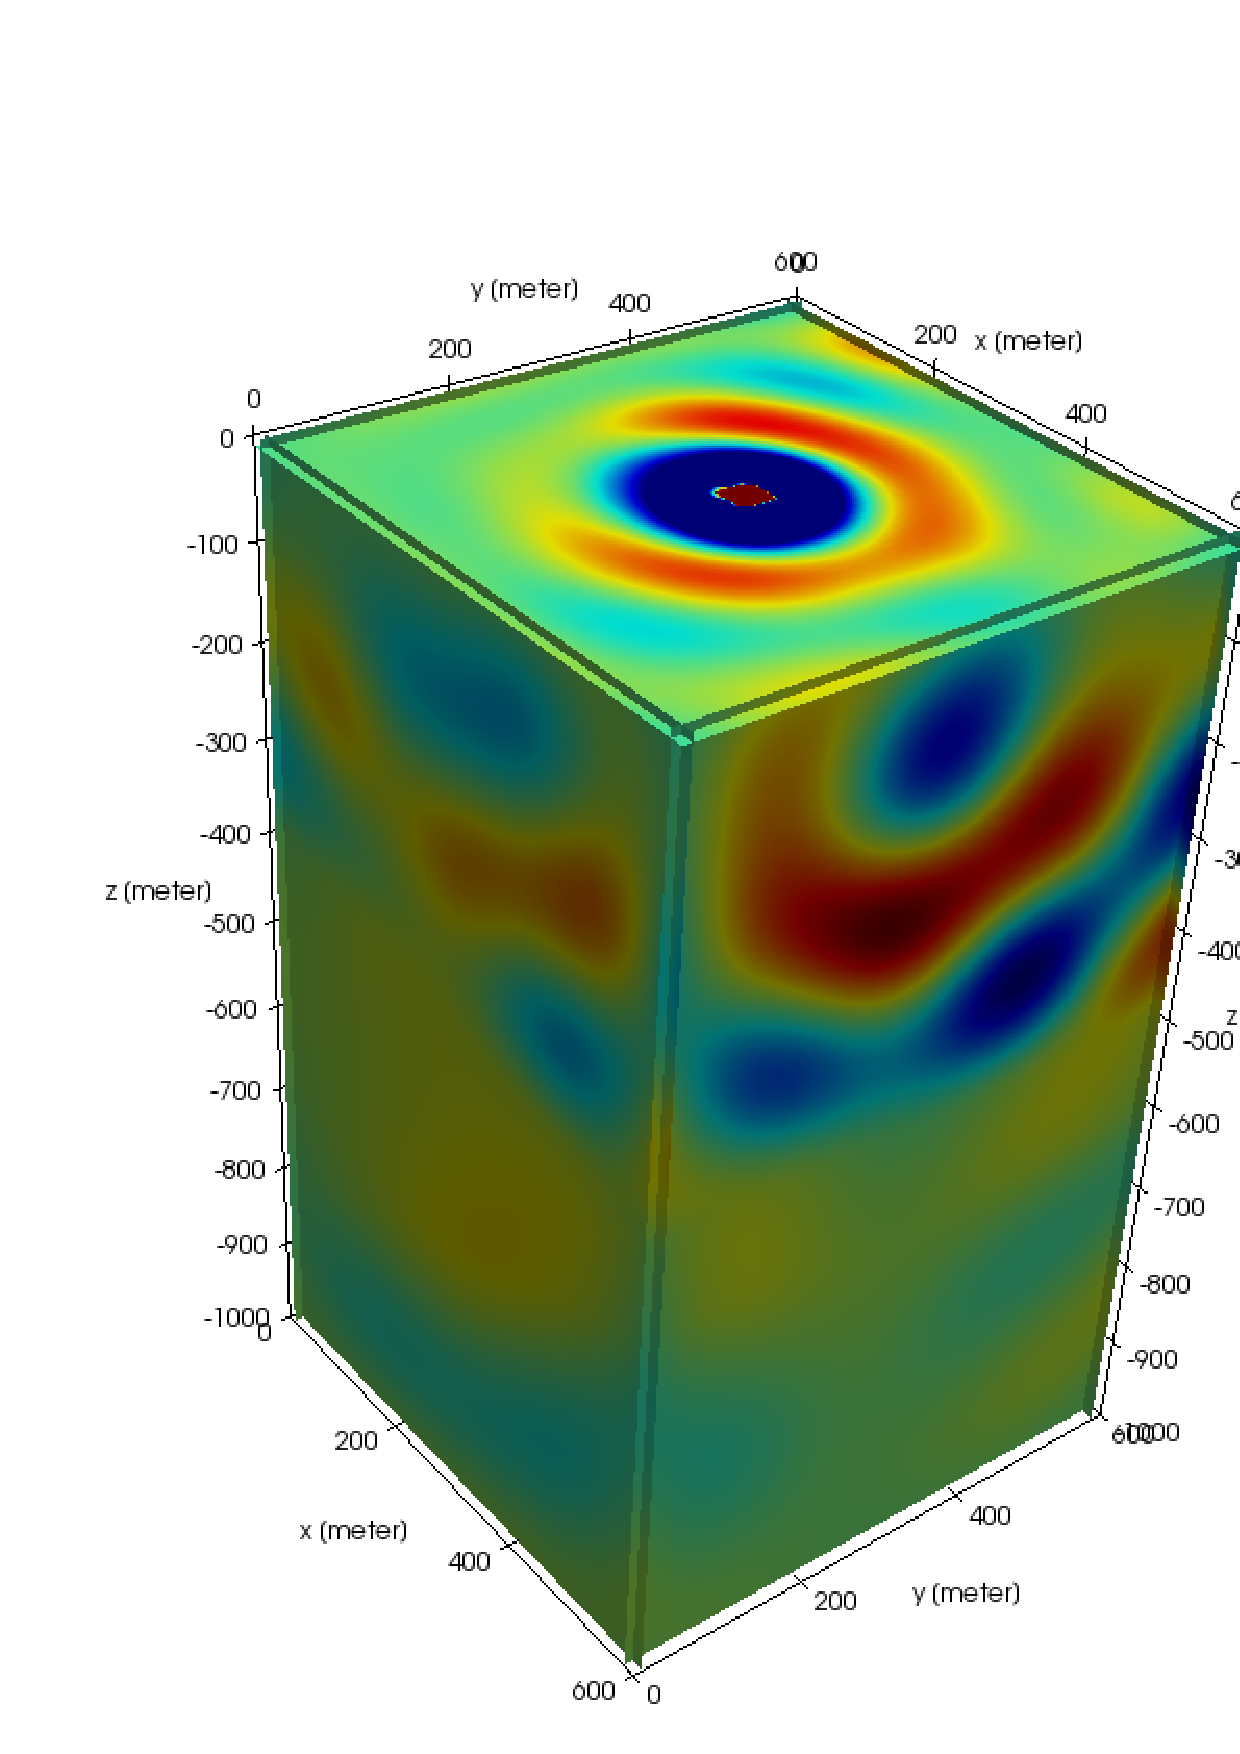
\includegraphics[width=0.49\columnwidth]{wedge3d_f4.png}
  \caption{Left: Parameter configuration of the elastic \texttt{wedge} problem for $d=3$ according to Table \ref{tab_params}. Right: Numerical solution of $\Re(\mathbf{u}_z)$ at $f= 4 Hz$.}\label{fig:3dwegdep1}
\label{fig:wedge3d_par}
\end{figure}

\begin{exper}[A 3D elastic wedge problem] \label{ex:num_3d}
A three-dim- ensional, inhomogeneous elastic wedge problem with physical parameters specified in Table \ref{tab_params} is solved using the SSOR-MSSS preconditioner described in Section \ref{ch_msss3d}.
\end{exper}

Similar to Experiment \ref{exp:freq1}, we consider a constant number of $20$ points per wavelength, and increase the wave frequency from $2$Hz to $4$Hz while doubling the number of grid points in each spatial direction. In Figure \ref{fig:3dwegdep1_conv} we observe a factor of $\sim 4$ which numerically indicates a complexity of $\mathcal{O}(n^5)$ for 3D problems. Moreover, we note that IDR outperforms BiCGStab in terms of number of iterations. The corresponding CPU times are presented in Table \ref{tab:cputime3d}: From the previous analysis, a factor of $\sim 32$ for the overall CPU times is expected since the number of unknowns in three spatial directions is doubled (linear complexity yields a factor of $8$), and Figure \ref{fig:3dwegdep1_conv} motivates an additional factor of $4$ in iteration numbers. 

 \begin{figure}[t]
 \centering
  \includegraphics[width=0.8\columnwidth]{wedge3d_f2_new3.pdf} \\
  \includegraphics[width=0.8\columnwidth]{wedge3d_f4_new2.pdf}
%   \includegraphics[width=0.8\columnwidth]{fig15/slobes.pdf} \\
%   \includegraphics[width=0.8\columnwidth]{fig15/slobes4.pdf}
  \caption{Convergence history of different Krylov methods preconditioned with the SSOR-MSSS preconditioner \eqref{eq:approx_Schur} for the 3D \texttt{wedge} problem of Figure \ref{fig:wedge3d_par}. We indicate (approximate) slopes based on a linear fit of the convergence curves.}\label{fig:3dwegdep1_conv}
 \end{figure}
 
\begin{table}[ht]
  \caption{Total CPU times in seconds corresponding to the convergence plots in Figure \ref{fig:3dwegdep1_conv}. Note that BiCGStab at \mbox{$f=4$ Hz} is stopped after $1,000$ iterations, cf. Figure \ref{fig:3dwegdep1_conv}.}\label{tab:cputime3d}
 \centering
 \begin{tabular}{|l|ccc|}
  \hline
  frequency & BiCGStab & IDR($4$) & IDR($16$)\\
  \hline
  $f=2$ Hz & \phantom{0}\texttt{144.5} & \phantom{00}\texttt{95.5} & \phantom{00}\texttt{91.3}\\
  $f=4$ Hz & \texttt{4430.7} & \texttt{3536.4} & \texttt{3100.5}\\
  \hline
 \end{tabular}
\end{table}
